\documentclass[aspectratio=169]{beamer}

% ── Theme ────────────────────────────────────────────────────────────────────
\usetheme{Madrid}
\usecolortheme{default}

% Custom color palette (deep teal + white + light grey)
\definecolor{primary}{RGB}{0, 90, 120}
\definecolor{accent}{RGB}{0, 150, 180}
\definecolor{lightgrey}{RGB}{245, 245, 245}

\setbeamercolor{palette primary}{bg=primary, fg=white}
\setbeamercolor{palette secondary}{bg=primary!80, fg=white}
\setbeamercolor{palette tertiary}{bg=primary!60, fg=white}
\setbeamercolor{palette quaternary}{bg=primary, fg=white}
\setbeamercolor{structure}{fg=primary}
\setbeamercolor{section in toc}{fg=primary}
\setbeamercolor{frametitle}{bg=primary, fg=white}
\setbeamercolor{title}{fg=white}
\setbeamercolor{block title}{bg=primary, fg=white}
\setbeamercolor{block body}{bg=lightgrey}
\setbeamercolor{alerted text}{fg=accent}

\setbeamertemplate{navigation symbols}{}
\setbeamertemplate{footline}{%
  \leavevmode%
  \hbox{%
    \begin{beamercolorbox}[wd=.45\paperwidth,ht=2.25ex,dp=1ex,left,leftskip=1em]{palette primary}%
      \usebeamerfont{author in head/foot}\insertshortauthor
    \end{beamercolorbox}%
    \begin{beamercolorbox}[wd=.45\paperwidth,ht=2.25ex,dp=1ex,center]{palette secondary}%
      \usebeamerfont{title in head/foot}\insertshorttitle
    \end{beamercolorbox}%
    \begin{beamercolorbox}[wd=.10\paperwidth,ht=2.25ex,dp=1ex,right,rightskip=1em]{palette primary}%
      \insertframenumber{} / \inserttotalframenumber
    \end{beamercolorbox}%
  }%
}

% ── Packages ─────────────────────────────────────────────────────────────────
\usepackage{graphicx}
\usepackage{booktabs}
\usepackage{multirow}
\usepackage{amsmath}
\usepackage{array}
\usepackage{tikz}
\usetikzlibrary{shapes.geometric, arrows.meta, positioning, fit, backgrounds, calc, trees}
\usepackage{xcolor}
\usepackage{colortbl}

% ── Helpers and TikZ Styles ─────────────────────────────────────────────────
\newcommand{\highlight}[1]{\textcolor{accent}{\textbf{#1}}}

% Colors used by CodeGraph tikz pictures
\definecolor{PrimaryTeal}{HTML}{005B7F}
\definecolor{AlertRed}{HTML}{D9534F}
\definecolor{WarningOrange}{HTML}{F0AD4E}
\definecolor{LightGray}{HTML}{F8F9FA}
\definecolor{BorderGray}{HTML}{E5E7EB}

\tikzset{
    box/.style={draw=primary, thick, fill=white, rounded corners=2pt, align=center, font=\small, minimum height=1cm, minimum width=2.5cm},
    highlightbox/.style={box, fill=primary!10},
    arr/.style={-{Stealth}, thick, draw=primary},
    seed/.style={circle, draw=AlertRed, fill=AlertRed!20, minimum size=0.6cm, font=\small},
    node/.style={circle, draw=primary, fill=primary!10, minimum size=0.6cm, font=\small},
    ranked/.style={circle, draw=WarningOrange, fill=WarningOrange!20, minimum size=0.6cm, font=\small}
}

% ── Metadata ─────────────────────────────────────────────────────────────────
\title[Repository-Level Structural Retrieval]{CodeGraph: Repository-Level Structural Retrieval for AI Coding Agents via Personalized PageRank}
\author[Toma Alexandru-Mihai]{Toma Alexandru-Mihai}
\institute[BBU]{%
  Department of Computer Science\\
  Babeș-Bolyai University\\[0.3em]
  Supervisor: Lect.\ PhD.\ Arthur Molnar
}
\date{2026\\[1.5em] \scriptsize \textit{Paper accepted at SCSS Conference 2026}}

% =============================================================================
\begin{document}
% =============================================================================

% ── Title slide ──────────────────────────────────────────────────────────────
\begin{frame}
  \titlepage
\end{frame}

% ── Outline ──────────────────────────────────────────────────────────────────
\begin{frame}{Outline}
  \hspace*{2em}\begin{minipage}{\dimexpr\textwidth-2em}
    {\setlength{\parskip}{1.2em}\tableofcontents}
  \end{minipage}
\end{frame}

\section{Motivation and Problem}
\begin{frame}{The Retrieval Bottleneck: Mismatch in Representation}
  \vspace{0.2cm}
  \begin{itemize}
    \setlength\itemsep{0.8em}
    \item \textbf{The Mismatch:} User requests are expressed in natural language, but codebases are organized through imports, calls, and inheritance.
    \item \textbf{The Limitation:} Standard lexical retrieval relies on surface-level similarity and can miss the target file completely.
    \item \textbf{The Consequence:} A retrieval bottleneck for AI coding agents when relevant code is \textit{structurally close but textually distant}.
  \end{itemize}
  
  \vspace{0.2cm}
  \centering
  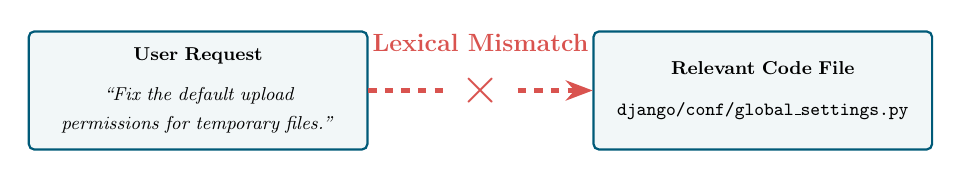
\begin{tikzpicture}[scale=0.75, transform shape]
    \node[box, fill=primary!5, draw=primary, text width=5.5cm, minimum height=2cm] (nl) {
      \textbf{User Request}\\
      \vspace{0.3cm}
      \small \textit{``Fix the default upload\\[0.1cm]permissions for temporary files.''}
    };
    
    \node[box, right=3.8cm of nl, fill=primary!5, draw=primary, text width=5.5cm, minimum height=2cm] (code) {
      \textbf{Relevant Code File}\\
      \vspace{0.3cm}
      \small \texttt{django/conf/global\_settings.py}
    };
    
    \draw[-{Stealth}, dashed, AlertRed, line width=1.5pt] (nl.east) -- node[midway, yshift=0.8cm, font=\bfseries\large, text=AlertRed] {Lexical Mismatch} node[midway, font=\Huge, text=AlertRed, fill=white, inner sep=2pt, circle] {$\times$} (code.west);
  \end{tikzpicture}
  
  \vspace{0.3cm}
  \begin{beamercolorbox}[rounded=true, shadow=true, sep=6pt, center, wd=0.95\textwidth]{palette primary}
    Surface similarity alone is not enough for repository-level retrieval.
  \end{beamercolorbox}
\end{frame}


\section{Why Code is a Graph}
\begin{frame}{Codebases as Connected Systems}
  \begin{columns}[T]
    \begin{column}{0.55\textwidth}
      \begin{itemize}
        \setlength\itemsep{0.8em}
        \item A codebase is not just a set of isolated files; it is a \textbf{connected system}.
        \item Functionality is distributed across files, classes, functions, imports, calls, and inheritance.
        \item Relevant context is better captured through \textbf{structural connections} than through keyword overlap.
      \end{itemize}
    \end{column}
    \begin{column}{0.4\textwidth}
      \begin{beamercolorbox}[rounded=true, shadow=true, sep=6pt, center]{palette primary}
        \small Code has a relational structure, not simply a flat directory.\\[0.2cm]
        \textbf{This is the conceptual foundation of CodeGraph.}
      \end{beamercolorbox}
    \end{column}
  \end{columns}
  
  \vspace{-0.4cm}
  \centering
  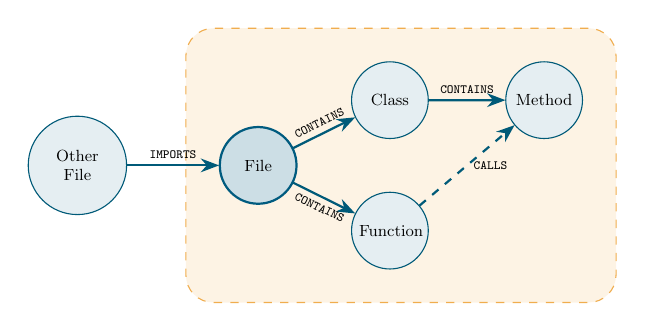
\begin{tikzpicture}[scale=0.65, transform shape]
    % Central cluster representing relevant neighborhood
    \node[node, fill=PrimaryTeal!20, draw=PrimaryTeal, thick, text width=1.2cm, align=center] (file) {File};
    \node[node, above right=0.2cm and 1.5cm of file, text width=1.2cm, align=center] (class) {Class};
    \node[node, below right=0.2cm and 1.5cm of file, text width=1.2cm, align=center] (func) {Function};
    \node[node, right=1.5cm of class, text width=1.2cm, align=center] (method) {Method};
    
    % Draw a highlight background
    \begin{scope}[on background layer]
        \node[fit=(file)(class)(func)(method), fill=WarningOrange!15, rounded corners=10pt, draw=WarningOrange, dashed, inner sep=12pt] (highlight) {};
    \end{scope}
    
    % Edges
    \draw[arr] (file) -- node[above, sloped, font=\scriptsize] {\texttt{CONTAINS}} (class);
    \draw[arr] (file) -- node[below, sloped, font=\scriptsize] {\texttt{CONTAINS}} (func);
    \draw[arr] (class) -- node[above, sloped, font=\scriptsize] {\texttt{CONTAINS}} (method);
    \draw[arr, dashed] (func) -- node[right, font=\scriptsize] {\texttt{CALLS}} (method);
    
    % External node
    \node[node, left=1.8cm of file, text width=1.5cm, align=center] (other) {Other\\File};
    \draw[arr] (other) -- node[above, font=\scriptsize] {\texttt{IMPORTS}} (file);
  \end{tikzpicture}
\end{frame}

\begin{frame}{Graph Database Schema}
  \begin{columns}[c]
    \begin{column}{0.45\textwidth}
      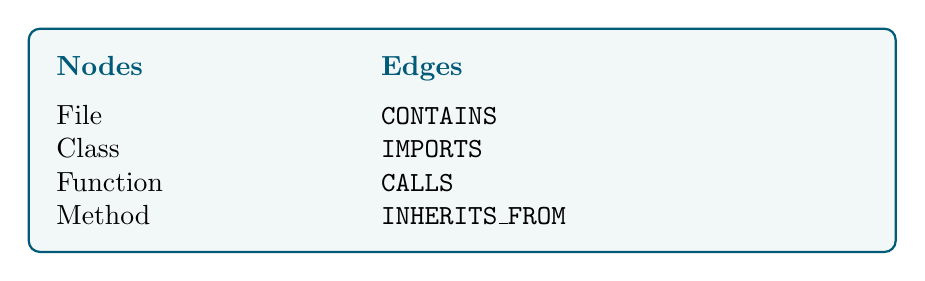
\begin{tikzpicture}
        \node[draw=primary, thick, fill=primary!5, rounded corners=4pt, inner sep=10pt, text width=0.85\linewidth] {
          \begin{minipage}[t]{0.4\linewidth}
            \vspace{0pt}
            \textbf{\textcolor{primary}{Nodes}}\\[0.2cm]
            File \\ Class \\ Function \\ Method
          \end{minipage}%
          \begin{minipage}[t]{0.55\linewidth}
            \vspace{0pt}
            \textbf{\textcolor{primary}{Edges}}\\[0.2cm]
            \texttt{CONTAINS} \\ \texttt{IMPORTS} \\ \texttt{CALLS} \\ \texttt{INHERITS\_FROM}
          \end{minipage}
        };
      \end{tikzpicture}
      
      \vspace{0.4cm}
      \footnotesize
      \begin{itemize}
        \item \textbf{Lightweight graph construction:} CodeGraph extracts the structural relations needed for retrieval without indexing every AST node.
        \item \textbf{Structural focus:} CodeGraph models the relations most useful for retrieval: calls, imports, and inheritance.
      \end{itemize}
    \end{column}
    
    \begin{column}{0.55\textwidth}
      \centering
      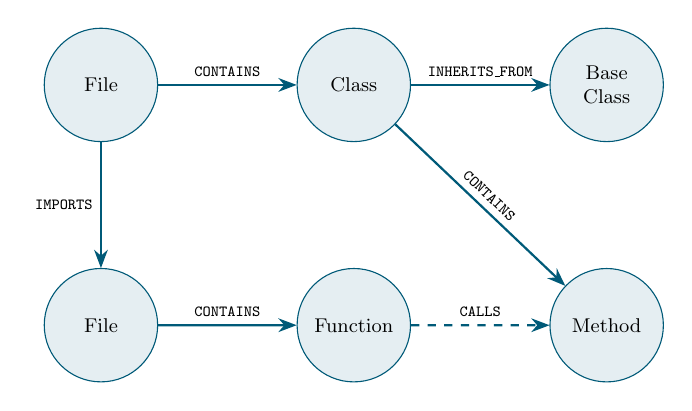
\begin{tikzpicture}[
          scale=0.8, transform shape,
          node distance=2.0cm and 2.2cm,
          circle_node/.style={node, align=center, text width=1.4cm, minimum size=1.8cm, inner sep=1pt}
        ]
        \node[circle_node] (file1) {File};
        \node[circle_node, below=of file1] (file2) {File};
        \draw[arr] (file1) -- node[left, font=\scriptsize] {\texttt{IMPORTS}} (file2);

        \node[circle_node, right=of file1] (class) {Class};
        \draw[arr] (file1) -- node[above, font=\scriptsize] {\texttt{CONTAINS}} (class);
        
        \node[circle_node, right=of class] (base) {Base\\Class};
        \draw[arr] (class) -- node[above, font=\scriptsize] {\texttt{INHERITS\_FROM}} (base);

        \node[circle_node, right=of file2] (func) {Function};
        \draw[arr] (file2) -- node[above, font=\scriptsize] {\texttt{CONTAINS}} (func);
        
        \node[circle_node, right=of func] (method) {Method};
        \draw[arr, dashed] (func) -- node[above, font=\scriptsize] {\texttt{CALLS}} (method);
        
        \draw[arr] (class) -- node[above, sloped, font=\scriptsize] {\texttt{CONTAINS}} (method);
      \end{tikzpicture}
    \end{column}
  \end{columns}
\end{frame}

\section{System Architecture}
\begin{frame}{CodeGraph System Overview}
  \centering
  \vspace{-0.2cm}
  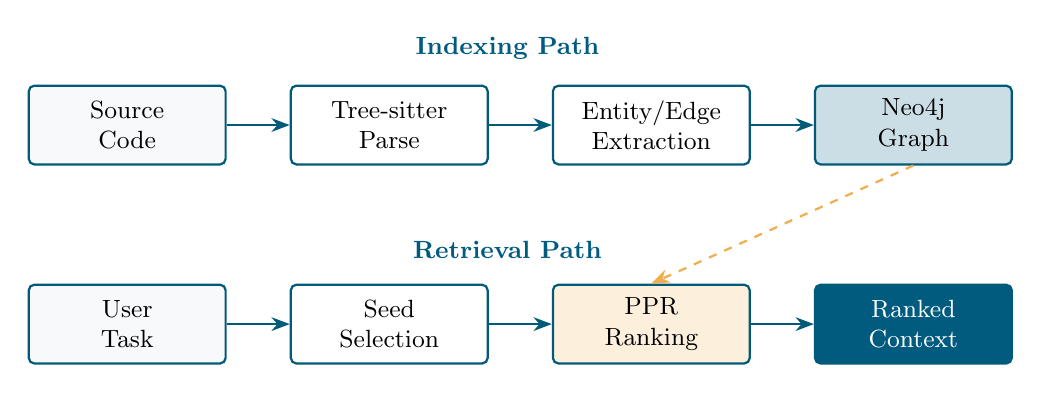
\begin{tikzpicture}[node distance=1cm and 0.8cm]
    % Indexing Path (Top row)
    \node[box, text width=2cm, fill=LightGray] (src) {Source\\Code};
    \node[box, right=of src, text width=2cm] (parse) {Tree-sitter\\Parse};
    \node[box, right=of parse, text width=2.2cm] (extract) {Entity/Edge\\Extraction};
    \node[box, right=of extract, text width=2cm, fill=PrimaryTeal!20] (neo4j) {Neo4j\\Graph};
    
    \draw[arr] (src) -- (parse);
    \draw[arr] (parse) -- (extract);
    \draw[arr] (extract) -- (neo4j);
    
    \node[above=0.2cm of parse, font=\bfseries\small, text=PrimaryTeal, xshift=1.5cm] {Indexing Path};

    % Retrieval Path (Bottom row)
    \node[box, below=1.5cm of src, text width=2cm, fill=LightGray] (task) {User\\Task};
    \node[box, right=of task, text width=2cm] (seed) {Seed\\Selection};
    \node[box, right=of seed, text width=2.2cm, fill=WarningOrange!20] (ppr) {PPR\\Ranking};
    \node[box, right=of ppr, text width=2cm, fill=PrimaryTeal, text=white] (payload) {Ranked\\Context};
    
    \draw[arr] (task) -- (seed);
    \draw[arr] (seed) -- (ppr);
    \draw[arr] (ppr) -- (payload);
    
    \node[above=0.2cm of seed, font=\bfseries\small, text=PrimaryTeal, xshift=1.5cm] {Retrieval Path};

    % Connection between phases
    \draw[arr, dashed, thick, draw=WarningOrange] (neo4j.south) -- (ppr.north);
  \end{tikzpicture}
  
  \vspace{0.5cm}
  \begin{columns}[c]
    \begin{column}{0.5\textwidth}
      \begin{itemize}
        \item \textbf{Indexing Path:} Translates source code into a static dependency graph.
        \item \textbf{Retrieval Path:} Uses lexical starting points and Personalized PageRank propagation.
      \end{itemize}
    \end{column}
    \begin{column}{0.45\textwidth}
      \begin{beamercolorbox}[rounded=true, shadow=true, sep=6pt, center]{palette primary}
        Deterministic, low-latency retrieval with\\ \textbf{no LLM in the retrieval loop}.
      \end{beamercolorbox}
    \end{column}
  \end{columns}
\end{frame}



\section{Related Work}
\begin{frame}{Related Work: Repository Context Retrieval}
  \vspace{0.4cm}
  \begin{itemize}
    \setlength\itemsep{0.6em}
    \item \textbf{CodexGraph:} Relies on LLMs to generate explicit database queries over a code graph. This introduces latency and depends heavily on the LLM's query-writing capabilities.
    \item \textbf{RepoGraph:} Retrieves repository context by expanding around local graph neighborhoods, but lacks a global, deterministic ranking algorithm over the entire topology.
    \item \textbf{Lexical \& Semantic Search:} Approaches like BM25 or vector embeddings are fast, but suffer from structural blindness and fail completely when vocabulary mismatches occur.
  \end{itemize}

  \vspace{0.4cm}
  \centering
  \begin{beamercolorbox}[rounded=true, shadow=true, sep=8pt, center, wd=0.95\textwidth]{palette primary}
    \textbf{Takeaway}\\
    Existing graph-based systems show that structure helps retrieval, but they leave open key trade-offs in ranking, determinism, and cost.
  \end{beamercolorbox}
\end{frame}

\section{Evaluation Setup}
\begin{frame}{Evaluation Setup: SWE-bench Lite}
  \textbf{A rigorous test of repository-level file localization on real-world data.}
  
  \vspace{0.3cm}
  \begin{itemize}
    \setlength\itemsep{1em}
    \item \textbf{The Benchmark:} 300 grounded GitHub issues drawn from 12 diverse, open-source Python repositories (e.g., \texttt{django}, \texttt{scikit-learn}).
    \item \textbf{The Retrieval Task:} Given only the natural-language issue description, retrieve the file modified in the human patch.
    \item \textbf{Evaluation Metric:} \textbf{Recall@10}. Does at least one target file appear in the top 10 ranked results?
  \end{itemize}
  
  \vspace{0.4cm}
  \centering
  \begin{beamercolorbox}[rounded=true, shadow=true, sep=8pt, center, wd=0.95\textwidth]{palette primary}
    \small SWE-bench Lite tests the exact scenario AI coding agents face:\\mapping abstract user intent to specific codebase files.
  \end{beamercolorbox}
\end{frame}

\section{Results}
\begin{frame}{Main Benchmark \& Ablation Results}
  \vspace{0.5cm}
  \centering
  \renewcommand{\arraystretch}{1.5}
  \begin{tabular}{@{}l c c@{}}
    \toprule
    \textbf{Retrieval Strategy} & \textbf{Recall@10} & \textbf{Delta} \\
    \midrule
    BM25-only Baseline & 49.7\% & -- \\
    Weighted PPR (Initial Baseline) & 42.0\% & -7.7\% \\
    Uniform PPR (Algorithm Refinement) & 60.7\% & +11.0\% \\
    \rowcolor{PrimaryTeal!15}
    \textbf{CodeGraph Optimal (+Seeds, $k=30$)} & \textbf{74.0\%} & \textbf{+24.3\%} \\
    \bottomrule
  \end{tabular}
  
  \vspace{0.4cm}
  \begin{beamercolorbox}[rounded=true, shadow=true, sep=8pt, center, wd=0.95\textwidth]{palette primary}
    \textbf{Takeaway}\\
    Leveraging deep code structure significantly improves retrieval performance over relying purely on lexical search.
  \end{beamercolorbox}
\end{frame}

\section{Discussion \& Conclusions}
\begin{frame}{Failure Analysis: The 78 Zero-Recall Cases}
  \textbf{Where is the absolute retrieval ceiling?}
  If lexical signals miss the correct structural neighborhood entirely, graph ranking alone cannot recover the target. \textbf{Seed reachability} is the true bottleneck.
  
  \vspace{0.8cm}
  \centering
  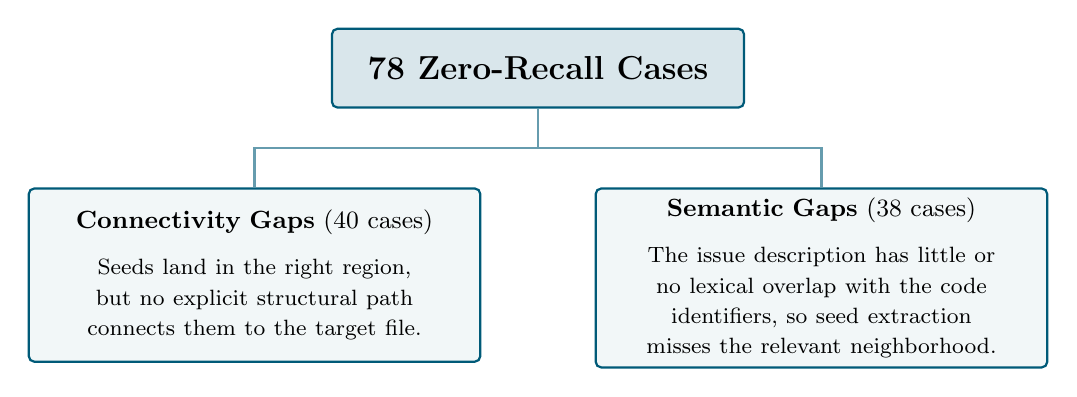
\begin{tikzpicture}[
      scale=1.0, transform shape,
      every node/.style={box, minimum height=2.2cm, text width=5.5cm}
    ]
    
    \node[fill=primary!15, draw=primary, text=black, font=\bfseries\large, text width=5cm, minimum height=1cm] (root) {78 Zero-Recall Cases};
    
    \coordinate (c_left) at ([xshift=-3.6cm, yshift=-1.0cm]root.south);
    \coordinate (c_right) at ([xshift=3.6cm, yshift=-1.0cm]root.south);
    
    \node[fill=primary!5, draw=primary, anchor=north] (gaps) at (c_left) {
      \textbf{Connectivity Gaps} (40 cases)\\
      \vspace{0.2cm}
      \footnotesize Seeds land in the right region, but no explicit structural path connects them to the target file.
    };
    
    \node[fill=primary!5, draw=primary, anchor=north] (semantic) at (c_right) {
      \textbf{Semantic Gaps} (38 cases)\\
      \vspace{0.2cm}
      \footnotesize The issue description has little or no lexical overlap with the code identifiers, so seed extraction misses the relevant neighborhood.
    };
    
    \draw[primary!60, thick] (root.south) -- +(0,-0.5) -| (gaps.north);
    \draw[primary!60, thick] (root.south) -- +(0,-0.5) -| (semantic.north);
  \end{tikzpicture}
\end{frame}

\begin{frame}{Live Demo}
  \vspace{0.5cm}
  \centering
  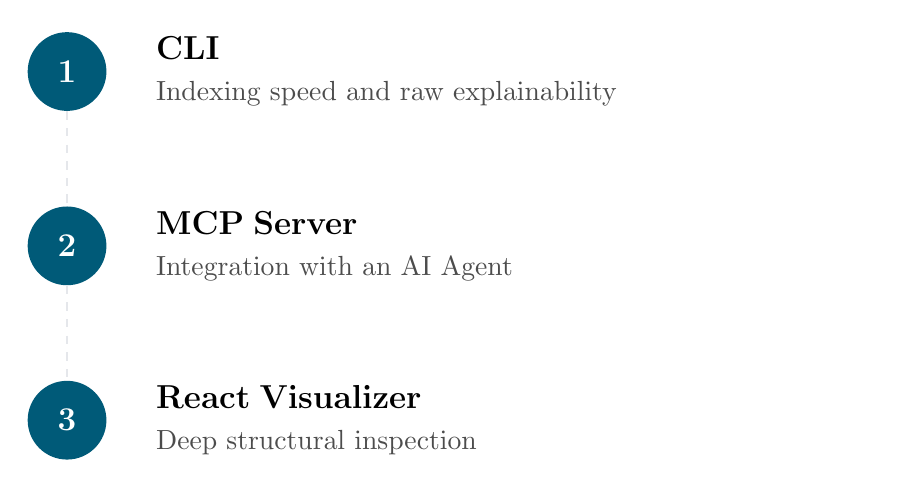
\begin{tikzpicture}[node distance=1.2cm]
    \node[circle, fill=primary, text=white, font=\bfseries\large, minimum size=1cm] (n1) {1};
    \node[right=0.5cm of n1, text width=9cm] (t1) {\large\textbf{CLI} \vspace{0.1cm}\\ \normalsize \textcolor{black!70}{Indexing speed and raw explainability}};
    
    \node[circle, fill=primary, text=white, font=\bfseries\large, minimum size=1cm, below=of n1] (n2) {2};
    \node[right=0.5cm of n2, text width=9cm] (t2) {\large\textbf{MCP Server} \vspace{0.1cm}\\ \normalsize \textcolor{black!70}{Integration with an AI Agent}};
    
    \node[circle, fill=primary, text=white, font=\bfseries\large, minimum size=1cm, below=of n2] (n3) {3};
    \node[right=0.5cm of n3, text width=9cm] (t3) {\large\textbf{React Visualizer} \vspace{0.1cm}\\ \normalsize \textcolor{black!70}{Deep structural inspection}};

    \begin{scope}[on background layer]
        \draw[thick, BorderGray, dashed] (n1) -- (n2);
        \draw[thick, BorderGray, dashed] (n2) -- (n3);
    \end{scope}
  \end{tikzpicture}
\end{frame}

\begin{frame}{Conclusions \& Future Work}
  \begin{columns}[T]
    \begin{column}{0.48\textwidth}
      \textbf{\large Conclusions}\\[0.3cm]
      \begin{itemize}
        \setlength\itemsep{1em}
        \item \textbf{Structure over Text:}\\Deterministic graph ranking (+24.3\%) significantly outperforms lexical baselines.
        \item \textbf{PPR is Essential:}\\Deep propagation is required; shallow expansion fails.
        \item \textbf{Inspectability:}\\The retrieval trace is mathematically verifiable.
      \end{itemize}
    \end{column}
    
    \begin{column}{0.48\textwidth}
      \textbf{\large Future Work}\\[0.3cm]
      \begin{itemize}
        \setlength\itemsep{1em}
        \item \textbf{Multi-Language Parsers:}\\Extending tree-sitter ingestion to TypeScript and Rust.
        \item \textbf{Dense Seed Selection:}\\Replacing exact-match/BM25 seeds with lightweight dense embeddings to solve Semantic Gaps.
        \item \textbf{Multi-Modal Edges:}\\Injecting git commit history and PR comments directly into the Neo4j graph structure.
      \end{itemize}
    \end{column}
  \end{columns}
\end{frame}

\begin{frame}
  \centering
  \vspace{1cm}
  {\Huge \textcolor{PrimaryTeal}{\textbf{Thank You}}}\\
  \vspace{1cm}
  {\Large Questions?}
\end{frame}

\begin{frame}{Relevant Bibliography}
  \small
  \begin{itemize}
    \setlength\itemsep{0.5em}
    \item Jimenez, C. E., et al. (2024). \textit{SWE-bench: Can Language Models Resolve Real-world Github Issues?} ICLR.
    \item Page, L., et al. (1999). \textit{The PageRank Citation Ranking: Bringing Order to the Web.} Stanford InfoLab.
    \item Robertson, S. \& Zaragoza, H. (2009). \textit{The Probabilistic Relevance Framework: BM25 and Beyond.}
    \item Brunsfeld, M., et al. (2024). \textit{Tree-sitter.}
    \item Ouyang, S., et al. (2025). \textit{RepoGraph: Enhancing AI Software Engineering with Repository-level Code Graph.} ICLR.
    \item Liu, X., et al. (2025). \textit{CodexGraph: Bridging LLMs and Code Repositories via Code Graph Databases.} NAACL.
  \end{itemize}
\end{frame}



\end{document}
